%! Author = joels
%! Date = 10/01/2022

\section{Checks}
\begin{itemize}[topsep=0pt]
    \itemsep -0.4em
    \item Separate good input from bad
    \item Information integrity checks
    \item Applied without complicating the program
\end{itemize}
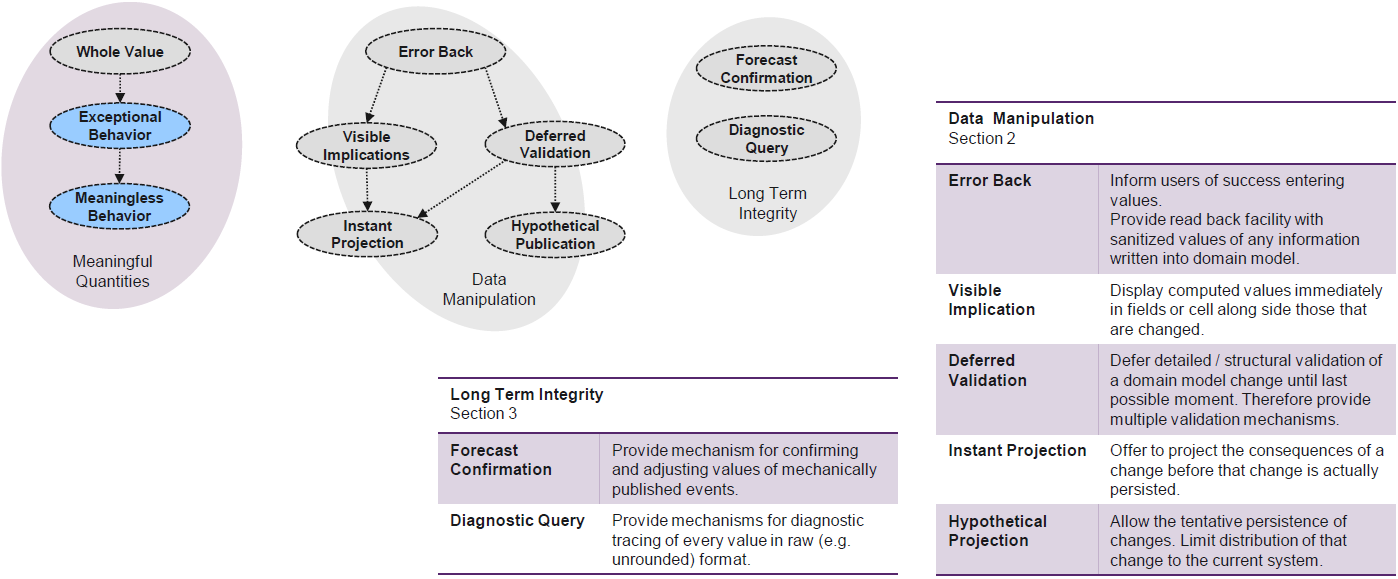
\includegraphics[width=\linewidth]{/checks_overview}

\subsection{Exceptional Behaviour}
\subsubsection{Problem}
\begin{itemize}[topsep=0pt]
    \itemsep -0.4em
    \item Missing or incorrect values in a domain model are impossible to avoid
    \item The domain logic should be able to handle this sort of missing data
    \item How can exceptional behaviour caused by invalid input be handled without throwing errors?
\end{itemize}
\subsubsection{Solution}
Use one or more distinguished values to represent exceptional circumstances.
\begin{itemize}[topsep=0pt]
    \itemsep -0.4em
    \item Invalid parametrized domain calls may produce Exceptional Values
    \item Domain logic may accept Exceptional Value as legal input
\end{itemize}
\begin{lstlisting}[style=htmlcssjs]
// TypeScript
export class Calculator {
  public static divide(numerator: number, divisor: number): number | CalculationError {
    if (divisor === 0) { return CalculationError.DivByZero; }
    if (isNaN(numerator)) { return CalculationError.NumeratorIsNaN; }
    if (isNaN(divisor)) { return CalculationError.DivisorIsNaN; }
    return numerator / divisor;
  }
}
\end{lstlisting}

\subsection{Meaningless Behaviour}
\subsubsection{Problem}
\begin{itemize}[topsep=0pt]
    \itemsep -0.4em
    \item Due to error handling, domain logic may be expressed with more complexity than originally conceived
    \item How can exceptional behaviour due to invalid input be handled without throwing errors?
\end{itemize}
\subsubsection{Solution}
Write methods with minimalistic concern for possible failure.
\begin{itemize}[topsep=0pt]
    \itemsep -0.4em
    \item Initiate computation
    \item If it fails:
        \SubItem recover from failure and continue processing
        \SubItem ensure the error is logged/visualized on surface
    \item Choose meaningless behaviour unless a condition has domain meaning 
    \item Represents an alternative implementation of Exceptional Value
\end{itemize}
\begin{lstlisting}[style=htmlcssjs]
// TypeScript
export class Calculator {
  public static divide(numerator: number, divisor: number): number {
  return numerator / divisor; // may result in Infinity (Java: NaN) if divisor is 0.0
  }
}
\end{lstlisting}

\section{Framework Introduction}
\textbf{Why Frameworks}
\begin{itemize}[topsep=0pt]
    \itemsep -0.4em
    \item Avoid re-inventing the wheel
    \item It is easy but inefficient to program the same thing again and again
\end{itemize}
\textbf{What is a Framework}
\begin{itemize}[topsep=0pt]
    \itemsep -0.4em
    \item Object-Oriented classes that work together $\rightarrow$ Many design patterns are microframeworks
    \item Framework provides \textit{hooks} for extension
    \item In contrast to a library, a framework keeps the control flow, not your extension $\rightarrow$ Inversion of control via callbacks
\end{itemize}
\textbf{Framework Callbacks}
\begin{itemize}[topsep=0pt]
    \itemsep -0.4em
    \item Hollywood Principle: Don't call us, we call you! $\rightarrow$ Control flow is from framework to application components
    \item Extendability and configurability
\end{itemize}
\subsection{Application Framework}
\begin{itemize}[topsep=0pt]
    \itemsep -0.4em
    \item Object-oriented class library
    \item \textit{Main()} program lives in the Application Framework
    \item Provides \textit{hooks} and \textit{callbacks}
    \item Provides ready-made classes for use
    \item Creates product families
    \item Reuse of application architecture and infrastructure
\end{itemize}
\subsection{Examples}
\textbf{Frameworks}
\begin{itemize}[topsep=0pt]
    \itemsep -0.4em
    \item .NET Core
    \item Entity Framework
    \item React (lib)
    \item Vue
\end{itemize}
\textbf{Application Framework}
\begin{itemize}[topsep=0pt]
    \itemsep -0.4em
    \item Spring
    \item ASP.NET
    \item Angular
\end{itemize}

\subsection{Difference: Library / Framework / App Framework}
\textbf{Library}
\begin{itemize}[topsep=0pt]
    \itemsep -0.4em
    \item Contain 3rd party Features which do not control the application flow (e.g. Math Library)
\end{itemize}
\textbf{Framework}
\begin{itemize}[topsep=0pt]
    \itemsep -0.4em
    \item Provide Hooks / Extension points
    \item Strogly rely on Inversion of Control (IoC) principle $\rightarrow$
    \item The framework defines when hooks (activities) are called thus controls part of the application flow
    \item E.g. JRE, .NET Fx, Vue, React
\end{itemize}
\textbf{App Framework}
\begin{itemize}[topsep=0pt]
    \itemsep -0.4em
    \item Contains the \textit{main()} procedure
    \item Clients implement plugins or components defined as extension points by the framework
    \item Completely controlls the app flow
    \item E.g. Spring Boot, ASP.NET, Angular
\end{itemize}

\subsection{Summary}
\textbf{Benefits}
\begin{itemize}[topsep=0pt]
    \itemsep -0.4em
    \item Less code to write
    \item Reliable and robust code
    \item Consistent and modular code
    \item Reusability
    \item Maintenance
\end{itemize}
\textbf{Liabilities}
\begin{itemize}[topsep=0pt]
    \itemsep -0.4em
    \item Portability: Code is strongly coupled to the overlying Framework 
    \item Testing: Close coupling between framework parts
    \item Evolution: User's implemetation may break due next Framework version
\end{itemize}

\subsection{Hook / Extension Point / Control Flow}
\subsubsection{Template Method}
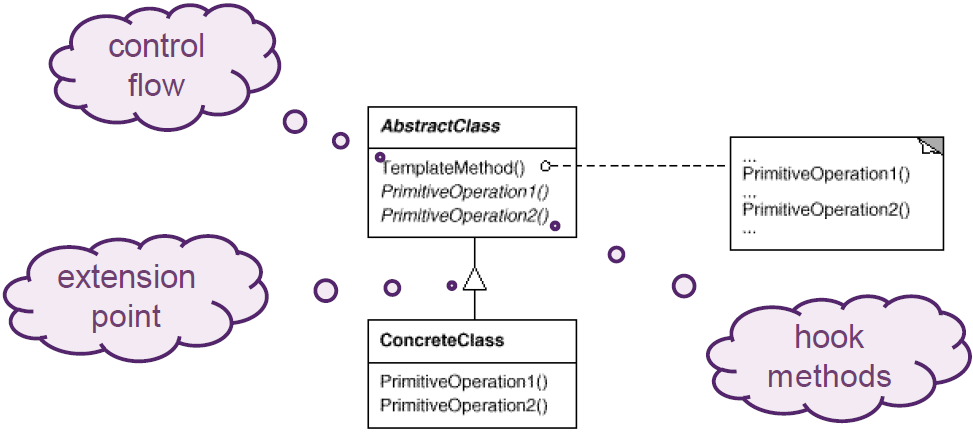
\includegraphics[width=\linewidth]{/template_method_example}
\subsubsection{Strategy}
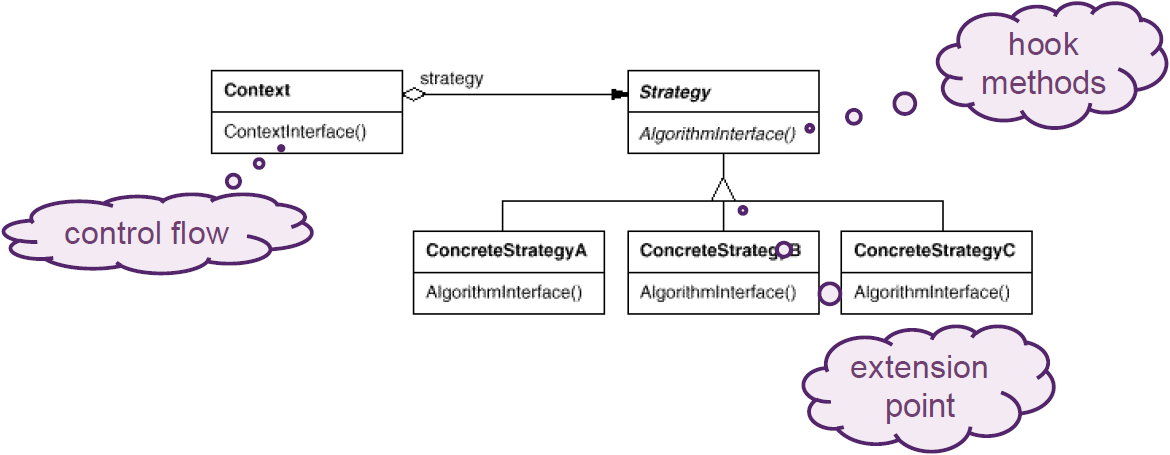
\includegraphics[width=\linewidth]{/strategy_example}
\subsubsection{Command Processor}
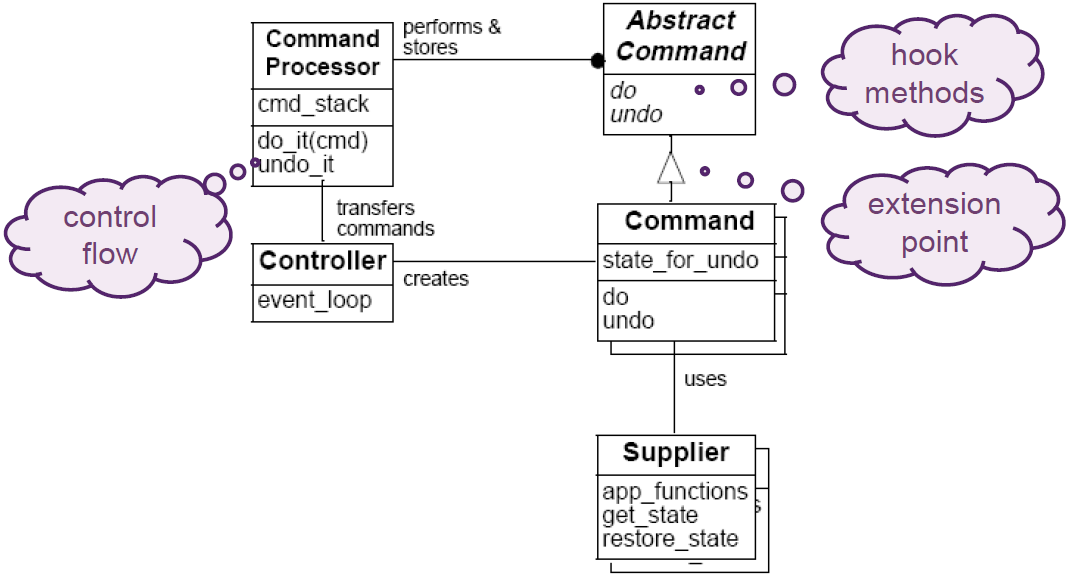
\includegraphics[width=\linewidth]{/command_processor_example}
\subsubsection{Flyweight}
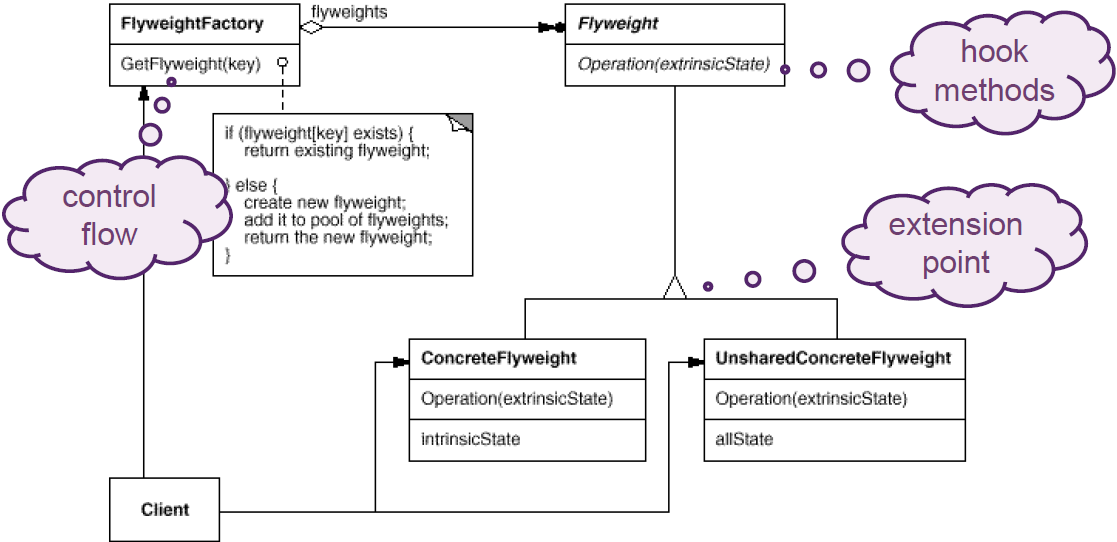
\includegraphics[width=\linewidth]{/flyweight_hooks}



\section{Meta Frameworks}
A Framework for Evaluating Software Technology
\begin{itemize}[topsep=0pt]
    \itemsep -0.4em
    \item Initial acquisition cost
    \item Long-term effect on quality, time to market, and cost of the organization’s products and services
    \item Training and support
    \item Relationship to future technoloy plans
    \item Response of direct competitor organizations
\end{itemize}

\subsection{Framework Evaluation Phases}
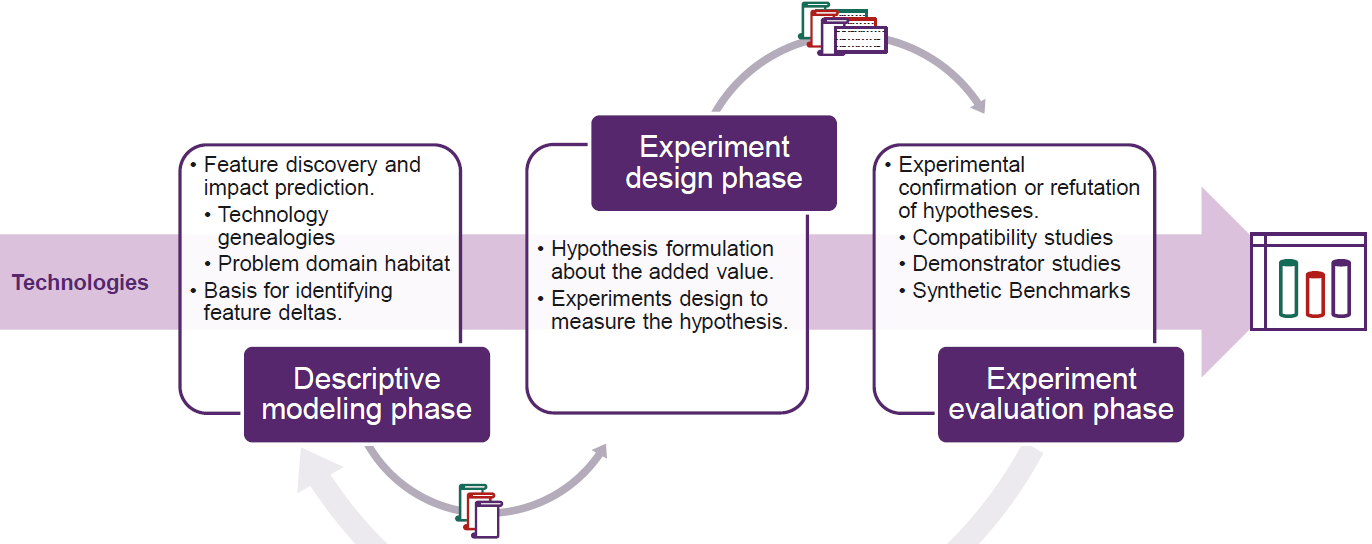
\includegraphics[width=\linewidth]{/framework_eval}

\section{Developing Frameworks}
\begin{itemize}[topsep=0pt]
    \itemsep -0.4em
    \item Frameworks need evolutionary improvements
\end{itemize}
\subsubsection{Frameworkers Dilemma}
\textbf{Potential ways out of the dilemma}
\begin{enumerate}[topsep=0pt]
    \itemsep -0.4em
    \item Think very hard up-front
    \item Don't care too much about framework users
    \item Let framework users participate
    \item Use helping technology
\end{enumerate}